\documentclass[10pt,aspectratio=43]{beamer}
\usepackage{multimedia}
\usepackage{graphicx}
\usepackage{xcolor}
\usepackage{pgfplots}
\pgfplotsset{compat=1.17}
\usetikzlibrary{positioning, shapes.geometric, arrows.meta}
\usepackage[normalem]{ulem} % For underlining in hyperlinks

% Define custom colors
\definecolor{myNewColorA}{RGB}{158, 27, 50} % Maroon-like color
\definecolor{myNewColorB}{RGB}{90, 27, 158} % Deep blue

% Beamer theme and color settings
\usetheme{CambridgeUS}
\usecolortheme{dolphin}

\setbeamercolor*{palette primary}{bg=myNewColorA, fg=white}
\setbeamercolor*{palette secondary}{bg=myNewColorB, fg=white}
\setbeamercolor*{palette tertiary}{bg=myNewColorA, fg=white}
\setbeamercolor*{titlelike}{fg=myNewColorA}
\setbeamercolor*{item}{fg=myNewColorA}
\setbeamercolor*{caption name}{fg=myNewColorA}
\setbeamerfont{title}{size=\Large}
\setbeamerfont{subtitle}{size=\small}
\setbeamerfont{author}{size=\small}
\setbeamerfont{date}{size=\footnotesize}
\setbeamerfont{institute}{size=\footnotesize}

% Fonts (requires LuaLaTeX or XeLaTeX for custom fonts)
\usepackage{fontspec}
\setmainfont{Times New Roman} % Default font; replace if needed

% TikZ styles
\tikzset{
    vertex/.style={
        circle,
        draw=black,
        fill=gray!20,
        thick,
        inner sep=0pt,
        minimum size=20pt
    },
    arrow/.style={
        -{Stealth[scale=1.2]},
        thick
    }
}

% Title and metadata
\title{Algorithms, Design \& Analysis}
\subtitle{Lecture 05: \textcolor{blue}{\textbf{Asymptotic Notations And Quick Sort}}}

\author[BSCS23177 & BSCS23095 ]{Hamza Raza And Fouz Ul Azeem}
\institute[ITU]{Information Technology University}
\date{\today}
\logo{\texorpdfstring{
\includegraphics[height=1cm]{figures/general/university_logo.png}}{}}

% Section transition slides
\AtBeginSection[]{
  \begin{frame}
    \vfill
    \centering
    \begin{beamercolorbox}[sep=8pt,center,shadow=true,rounded=true]{title}
      \usebeamerfont{title}\insertsectionhead
    \end{beamercolorbox}
    \vfill
  \end{frame}
}

\begin{document}

\begin{frame}
    \titlepage
\end{frame}

% Include external content
\setmainfont{Noteworthy}
%TODO: provide your details here.
\begin{frame}
    \frametitle{About Your Fellows}
    \begin{itemize}
        \item Hi there! We are \textcolor{blue}{\textbf{ Assadullah Farrukh}  \textcolor{black}{and}\textbf{ M.Hamza Naveed}}.
        \item We are Associate Students at ITU.
    \end{itemize}
\end{frame}




\begin{frame}
    \frametitle{Recap}
    \begin{itemize}
        \item Problem: \textcolor{red}{Find the kth smallest element in a distinct array?}
    \end{itemize}
\end{frame}

\begin{frame}
    \frametitle{Recap}
    \vspace{0.3cm} % Adds spacing for better visual appearance
    \begin{itemize}
        \item \textbf{Problem:} \textcolor{red}{Find the k\textsuperscript{th} smallest element in an array with distinct elements.}
        \vspace{0.3cm} % Adds spacing between items
        \item \textcolor{blue}{\textbf{Algorithm 1:}}
        \vspace{0.2cm} % Adds spacing before the sub-item list
        \begin{itemize}
            \item \textcolor{black}{Find the smallest  element in the array, remove it, and store it in a variable.}
            \item \textcolor{black}{Repeat this process \textbf{k} times.}
            \item \textcolor{black}{The value in the variable after the \textbf{k\textsuperscript{th}} iteration is the \textbf{k\textsuperscript{th}} smallest element.}
        \end{itemize}
         \item \textbf{Time Complexity:} \textit{O(kN)}, where \textit{N} is the size of the array.
    \end{itemize}
    \vspace{0.5cm} % Adds spacing at the bottom of the slide for a clean look
\end{frame}

\begin{frame}
    \frametitle{Recap}
    \vspace{0.3cm} % Adds spacing for better visual appearance
    \begin{itemize}
        \item \textbf{Problem:} \textcolor{red}{Find the k\textsuperscript{th} smallest element in an array with distinct elements.}
        \vspace{0.3cm} % Adds spacing between items
        \item \textcolor{blue}{\textbf{Algorithm 2:}}
        \vspace{0.2cm} % Adds spacing before the sub-item list
        \begin{itemize}
            \item \textcolor{black}{Do Merge sort in the array}
            \item \textcolor{black}{Return the element at the \textbf{(k-1)\textsuperscript{th}} index of the array.}
        \end{itemize}
         \item \textbf{Time Complexity:} \textit{O(Nlog(N))}, where \textit{N} is the size of the array.
    \end{itemize}
    \vspace{0.5cm} % Adds spacing at the bottom of the slide for a clean look
\end{frame}

\begin{frame}
    \frametitle{Recap}
    \vspace{0.3cm} % Adds spacing for better visual appearance
    \begin{itemize}
        \item \textbf{Problem:} \textcolor{red}{Find the k\textsuperscript{th} smallest element in an array with distinct elements.}
        \vspace{0.3cm} % Adds spacing between items
        \item \textcolor{blue}{\textbf{Algorithm 3: \textcolor{teal}{Guess Select Algorithm (}\textcolor{cyan}{commonly known as the} \textcolor{orange}{Randomized Select Algorithm}\textcolor{teal}{)}}}
        \vspace{0.2cm} % Adds spacing before the sub-item list
        \begin{itemize}
            \item \textcolor{black}{\textbf{Input:} Array \textit{A} and \textit{k}, where \textit{k} is the position of the desired element.}
            \item \textcolor{black}{Guess \textit{g} as an element from \textit{A}. Uniformly Randomly pick a number.}
            \item \textcolor{black}{Partition \textit{A} into:}
            \begin{itemize}
                \item \textit{L}: Elements less than \textit{g}.
                \item \textit{R}: Elements greater than \textit{g}.
            \end{itemize}
            \item \textcolor{black}{Compute the rank of \textit{g} using \textit{L} and \textit{R}.}
            \item \textcolor{black}{If $|L| = k-1$, return \textit{g}.}
            \item \textcolor{black}{Else if $|L| > k$, recursively select \textit{k\textsuperscript{th}} element from \textit{L}.}
            \item \textcolor{black}{Otherwise, recursively select \textit{(k - |L| - 1)\textsuperscript{th}} element from \textit{R}.}
        \end{itemize}
    \end{itemize}
    \vspace{0.5cm} % Adds spacing at the bottom of the slide for a clean look
\end{frame}


\begin{frame}
    \frametitle{Types of Algorithms}
    \vspace{0.4cm} % Adds spacing for better visual balance
    
        Randomized algorithms can be classified into two main types:
    \vspace{0.4cm} % Adds spacing between the block and the list

    \begin{itemize}
        \item \textbf{\textcolor{blue}{Monte Carlo Algorithm}}
        \vspace{0.3cm} % Adds spacing between items for readability
        
        \item \textbf{\textcolor{blue}{Las Vegas Algorithm}}
    \end{itemize}
    
    \vspace{0.5cm} % Adds spacing at the bottom of the slide for a clean look
\end{frame}


\begin{frame}
    \frametitle{Monte Carlo Algorithm}
    \vspace{0.4cm} % Adds spacing for better visual balance
    
    \begin{block}{\textcolor{red}{Characteristics}}
        - Stops in a fixed amount of time but does not guarantee a result. \\
        - The outcome is probabilistic, relying on randomness.
    \end{block}
    \vspace{0.4cm} % Adds spacing between the block and the list

    \begin{itemize}
        \item \textbf{\textcolor{blue}{Fixed Runtime:}} 
        Executes within a pre-determined, fixed duration regardless of input size.
        \vspace{0.3cm} % Adds spacing between items for readability
        
        \item \textbf{\textcolor{blue}{Randomized Outcome:}} 
        The result is a random variable and may not always be found.
    \end{itemize}
    
    \vspace{0.5cm} % Adds spacing at the bottom of the slide for a clean, symmetrical appearance
\end{frame}


\begin{frame}
    \frametitle{Las Vegas Algorithm}
    \vspace{0.4cm} % Adds spacing for better visual balance
    
    \begin{block}{\textcolor{red}{Characteristics}}
        - Always produces a correct result, but runtime is not fixed. \\
        - The execution time depends on randomness and may vary.
    \end{block}
    \vspace{0.4cm} % Adds spacing between the block and the list

    \begin{itemize}
        \item \textbf{\textcolor{blue}{Guaranteed Correctness:}} 
        The algorithm always delivers a correct result, regardless time taken.
        \vspace{0.3cm} % Adds spacing between items for readability
        
        \item \textbf{\textcolor{blue}{Variable Runtime:}} 
        The runtime can fluctuate depending on the random choices made during execution.
    \end{itemize}
    
    \vspace{0.5cm} % Adds spacing at the bottom of the slide for a clean, symmetrical appearance
\end{frame}


\begin{frame}
    \frametitle{Optimality of Las Vegas Algorithm}
    \vspace{0.4cm} % Adds spacing for better visual balance

    \begin{block}{\textcolor{red}{Which Algorithm is Optimal?}}
        Oh, the \textbf{Las Vegas Algorithm} is optimal! But why? Let's find out.
    \end{block}
    \vspace{0.4cm} % Adds spacing between the block and the explanation

    \begin{itemize}
        \item \textbf{\textcolor{blue}{Why is it Optimal?}} 
        Because we \textbf{do not stop until the job is done}. The algorithm keeps running until it produces a \textbf{correct result}.
        \vspace{0.3cm} % Adds spacing between items for readability
        
        \item \textbf{\textcolor{blue}{Guaranteed Accuracy:}} 
        Since the algorithm doesn't terminate until it finds a valid solution, the outcome is always \textbf{correct and reliable}.
    \end{itemize}
    
    \vspace{0.5cm} % Adds spacing at the bottom for a clean look
\end{frame}


\begin{frame}
    \frametitle{Algorithm Used in Randomized Select}
    \vspace{0.4cm} % Adds spacing for better visual balance
     \textcolor{red}{Which Algorithm was used in yesterday's randomized select algorithm?}
    
    \vspace{0.5cm} % Adds spacing at the bottom for a clean look
\end{frame}


\begin{frame}
    \frametitle{Algorithm Used in Randomized Select}
    \vspace{0.4cm} % Adds spacing for better visual balance

    \begin{block}{\textcolor{red}{Which Algorithm was used in yesterday's randomized select algorithm?}}
        The \textbf{Las Vegas Algorithm} was used in yesterday's Randomized Select Algorithm!
    \end{block}
    \vspace{0.4cm} % Adds spacing between the block and the explanation

    \begin{itemize}
        \item \textbf{\textcolor{blue}{Why Las Vegas Algorithm?}} 
        Because it \textbf{provides a guaranteed solution}, ensuring correctness in the result.
        \vspace{0.3cm} % Adds spacing between items for readability
        
        \item \textbf{\textcolor{blue}{Reliability:}} 
        Unlike Monte Carlo algorithms, Las Vegas algorithms \textbf{never compromise on accuracy}, making them ideal for Randomized Select.
    \end{itemize}
    
    \vspace{0.5cm} % Adds spacing at the bottom for a clean, symmetrical look
\end{frame}


\begin{frame}
    \frametitle{Worst-Case Time Complexity of Randomized Select}
    \vspace{0.4cm} % Adds spacing for better visual balance

    \begin{block}{\textcolor{red}{What is the Worst Case?}}
        The worst-case scenario occurs when the algorithm repeatedly selects the \textbf{least optimal pivot}, leading to unbalanced partitions.
    \end{block}
    \vspace{0.4cm} % Adds spacing between the block and the explanation

    \begin{itemize}
        \item \textbf{\textcolor{blue}{Worst-Case Time Complexity:}} 
        In the worst case, the time complexity of our Randomized Select becomes \textbf{O(n²)}. This happens when each partitioning step reduces the problem size by only one element.
        \vspace{0.3cm} % Adds spacing between items for readability
        
        \item \textbf{\textcolor{blue}{Why Does This Happen?}} 
        The random pivot selection may consistently divide the array unevenly, causing the algorithm to behave like a naive selection algorithm.
    \end{itemize}
    
    \vspace{0.5cm} % Adds spacing at the bottom for a clean, symmetrical look
\end{frame}


\begin{frame}
    \frametitle{Worst-Case Time Complexity Derivation}
    \vspace{0.3cm}

    \begin{block}{\textcolor{red}{Recursive Relation}}
        The recurrence relation for the worst-case time complexity of Randomized Select is:
        \[
        \textbf{T(n) = cn + T(n-1)}
        \]
        \textit{where \(c\) is a constant representing the time taken for partitioning.}
    \end{block}
    \vspace{0.4cm}

    \begin{block}{\textcolor{blue}{Base Case}}
        \[
        \textbf{T(1) = a}
        \]
        \textit{where \(a\) is a constant representing the time for the smallest input size.}
    \end{block}
    \vspace{0.4cm}

\end{frame}
\begin{frame}
    \frametitle{Worst-Case Time Complexity Derivation}
    \vspace{0.3cm}
    \begin{block}{\textcolor{teal}{Derivation}}
        Expanding the recurrence:
        \[
        T(n) = cn + c(n-1) + c(n-2) + \dots + c(1) + a
        \]
        Simplifies to:
        \[
        T(n) = c \sum_{i=1}^{n} i + a = c \frac{n(n+1)}{2} + a
        \]
        \textbf{Resulting in the Worst-Case Complexity: \(T(n) = O(n^2)\).}
    \end{block}

    \vspace{0.6cm}
    \hrule % Adds a decorative horizontal line at the bottom
    \centering
    \vspace{0.2cm}☻☻
    \textit{\textcolor{gray}{The worst case occurs when the pivot selection repeatedly divides unevenly causing the size to only go down by 1.}}

\end{frame}


\begin{frame}
    \frametitle{Professor's Question}
    \vspace{0.4cm} % Adds spacing for better visual balance

    \begin{block}{\textcolor{red}{Question:}}
        The professor asked the class:
        \begin{center}
            \textit{\textbf{What is the average runtime of an Algorithm?}}
        \end{center}
    \end{block}
    
    \vspace{0.6cm} % Adds spacing for a clean bottom look
    \begin{center}
        \textit{\textcolor{gray}{The class was quiet, thinking... until Wasif spoke up.}}
    \end{center}
\end{frame}



\begin{frame}
    \frametitle{Wasif's Reply}
    \vspace{0.4cm} % Adds spacing for better visual balance

    \begin{block}{\textcolor{blue}{Wasif's Response:}}
        Wasif hesitantly replied:
        \vspace{0.4cm}

            \textbf{Average Runtime:} \quad 
        \begin{center}
            \[
            \frac{\text{Best Case} + \text{Worst Case}}{2}
            \]
        \end{center}
    \end{block}

    \vspace{0.6cm} % Adds spacing for a clean bottom look
    \begin{center}
        \textit{\textcolor{gray}{The professor smiled, but was it the correct answer?}}
    \end{center}
\end{frame}


\begin{frame}
    \frametitle{Derivation of Average Runtime}
    \vspace{0.4cm}

    \begin{block}{\textcolor{blue}{Derivation Steps:}}
        \textbf{1. Average Runtime:} \( \frac{\text{Best Case} + \text{Worst Case}}{2} \)

        \vspace{0.3cm}
        \textbf{2. Recurrence Relation for Best Case:} \( T(n) = cn + T\left(\frac{n}{2}\right) \)

        \vspace{0.3cm}
        \textbf{3. Expanding Recurrence:}
        \[
        T(n) = cn + c\frac{n}{2} + c\frac{n}{4} + \dots + 2
        \]

        \vspace{0.3cm}
        \textbf{4. Summing Series:}
        \[
        T(n) = a + cn \sum_{i=1}^k \left(\frac{1}{2}\right)^i
        \]

        \vspace{0.3cm}
        \textbf{5. Simplifying:} \( \leq a + 2cn = O(n) \)
    \end{block}

\end{frame}

\begin{frame}
    \frametitle{Derivation of Average Runtime}
    \vspace{0.4cm}
    \begin{block}
        
        \vspace{0.3cm}
        \textbf{6. Combining Best and Worst:}
        \[
        \frac{O(n^2) + O(n)}{2} = O(n^2)
        \]
    \end{block}

    \vspace{0.4cm}
    \begin{center}
        \textit{\textcolor{gray}{The derivation concludes that the average runtime is \( O(n^2) \) which is the same as the worst case runtime so this can't be right Professor appreciated Wasif for his try moved on to explain what Average run time actually is by giving a hint that it is also called expected average runtime.}}
    \end{center}
\end{frame}

\begin{frame}
    \frametitle{Expected Average Time Complexity}
    \vspace{0.4cm}

    \begin{block}{\textcolor{blue}{Expected Runtime Derivation:}}
        \textbf{1. Average Runtime (Expected):}
        \[
        \mathbb{E}(T(n)) = Cn + T(\mathbb{E}(L)) \quad \text{or} \quad \mathbb{E}(T(n)) = Cn + T(\mathbb{E}(R))
        \]
        
        \textbf{2. Explanation:}
        \begin{itemize}
            \item The expected time complexity is the time taken by using expectation so now the recursive relation is like this as the next recursion will be for the $L$ or $R$ which ever is now supposed to have the kth value.
        \end{itemize}

        \vspace{0.3cm}
  
    \end{block}

    \vspace{0.4cm}
    \begin{center}
        \textit{\textcolor{gray}{Now all of our faces showed the Professor like he had lost us some where so...}}
    \end{center}
\end{frame}

\begin{frame}
    \frametitle{Expectation: A Class Discussion}
    \vspace{0.3cm}

    \begin{block}{\textcolor{red}{The Question}}
        The professor asked the class:
        \begin{center}
            \textbf{"You do know what expectation and random variables are?"}
        \end{center}
        \textit{But despite knowing the answer, no one could recall what even those words were!}
    \end{block}
    \vspace{0.4cm}

    \begin{block}{\textcolor{blue}{Professor's Explanation}}
        The professor began explaining the concept of expectation, step by step. The curiosity in the room grew!
    \end{block}
    \vspace{0.4cm}

\end{frame}

\begin{frame}
    \frametitle{Example: Coin Toss Experiment}
    \vspace{0.3cm}

    \begin{block}{\textcolor{red}{Scenario}}
        Consider the random variable \(X\): the number of heads in the toss of two coins. Possible values are \(0, 1, 2\).
    \end{block}
    \vspace{0.4cm}

    \begin{block}{\textcolor{blue}{Probability Distribution}}
        \[
        \mathcal{P}(X = 0) = \frac{1}{4}, \quad \mathcal{P}(X = 1) = \frac{1}{2}, \quad \mathcal{P}(X = 2) = \frac{1}{4}
        \]
    \end{block}

\end{frame}

\begin{frame}
    \frametitle{Expected Value Calculation}
    \vspace{0.3cm}

    \begin{block}{\textcolor{red}{Calculation}}
        Using the formula:
        \[ \mathbb{E}(X) = 0 \cdot \mathcal{P}(X=0) + 1 \cdot \mathcal{P}(X=1) + 2 \cdot \mathcal{P}(X=2) \]
        \[ \mathbb{E}(X) = 0 \cdot \frac{1}{4} + 1 \cdot \frac{1}{2} + 2 \cdot \frac{1}{4} = 1 \]
    \end{block}
    \vspace{0.4cm}

    \begin{block}{\textcolor{blue}{Conclusion}}
        The expected number of heads is \textbf{1} in two coin tosses.
    \end{block}

\end{frame}

\begin{frame}
    \frametitle{The Formula of Expectation}
    \vspace{0.3cm}

    \begin{block}{\textcolor{red}{Definition of Expectation}}
        The professor wrote the formula for expectation:
        \[ \mathbb{E}(X) = \sum_{i} x_i \cdot \mathcal{P}(x_i) \]
    \end{block}
    \vspace{0.4cm}

    \begin{block}{\textcolor{blue}{Class Reaction}}
        More than half of the class suddenly exclaimed:
        \begin{center}
            \textbf{"Oh yeah, we know this!"}
        \end{center}
    \end{block}
    \vspace{0.4cm}

\end{frame}

\begin{frame}
    \frametitle{Back to Expected Average Time Calculation}
    \begin{itemize}
        \item Recurrence Relation:
        \[
        \mathbb{E}(T(n)) = Cn + T(\mathbb{E}(L)) \quad \text{or} \quad \mathbb{E}(T(n)) = Cn + T(\mathbb{E}(R))
        \]
        \item Assumption: \(L\) is always the smallest among the partitions \(L\) and \(R\).
        \[
        T(n) = cn + T(|L|)
        \]
        \item Sorted Array:
        \[
        a_1, a_2, \dots, a_n
        \]
        \item If \(k\) is the median, then \(g\) is a good guess only if the array \(A\) was sorted. In that case, the guess lies between \(a_{n/4} \) and \(a_{3n/4}\).
    \end{itemize}
\end{frame}

\begin{frame}
    \frametitle{Back to Expected Average Time Calculation}
    \begin{itemize}
        \item Guessing Method:
        \[
        \mathcal{P}\left(g \in \left(a_{\frac{n}{4}}, a_{\frac{3n}{4}}\right)\right) = \frac{1}{2}
        \]
        If you are willing to see how this \(\frac{1}{2}\) came,    
        \href{https://drive.google.com/file/d/1DqlktCr-hvTREOOm8hhHVSO5Sv6QmoWf/view?usp=sharing}{\color{blue}{\underline{click here}}.}
    
        \item Expected Value:
        \[
        \mathbb{E} = \frac{1}{\mathcal{P}}
        \]
        \[
        \mathbb{E}(w) = 2
        \]
        \item Therefore, it is expected to take 2 guesses to find \(g\) such that it is a good guess within the range \(\left(a_{\frac{n}{4}}, a_{\frac{3n}{4}}\right)\).
    \end{itemize}
\end{frame}


\begin{frame}
    \frametitle{Expected Recurrence Analysis}
    \begin{itemize}
        \item Recurrence for \(T(n)\):
        \[
        \mathbb{E}(T(n)) = c \cdot 2 \cdot n + T\left(\frac{3n}{4}\right)
        \]
        \item The \( \frac{3n}{4} \) term appears because, in the worst case, even if the guess was a good guess, the larger partition (assumed to be \(L\)) could still contain \(\frac{3n}{4}\) elements.
        \vspace{0.4cm}
        \item Expanding the recurrence:
        \[
        \mathbb{E}(T(n)) = c \cdot 2 \cdot n + c \cdot 2 \cdot \frac{3n}{4} + c \cdot 2 \cdot \left(\frac{3}{4}\right)^2 n + \dots
        \]
            \end{itemize}
\end{frame}
\begin{frame}
    \frametitle{Expected Recurrence Analysis}
    \begin{itemize}
        \item This forms a geometric series with a common ratio of \(\frac{3}{4}\):
        \[
        \sum_{i=0}^{\infty} \left(\frac{3}{4}\right)^i \leq 4
        \]
        \item Simplifying the series:
        \[
        T(n) \leq O(n)
        \]
        \vspace{0.2cm}
        \item Thus, even in the worst case where the good guess leads to an imbalance, the overall time complexity remains linear.
    \end{itemize}
\end{frame}

\begin{frame}
    \frametitle{Median of Medians Algorithm For Selection}
    \begin{enumerate}
        \item Divide array \(A\) into chunks of size 5.
        \[
        A_1, A_2, A_3, \dots, A_{\lceil n/5 \rceil}
        \]
        \item Find the median of each chunk using insertion sort.
        \[
        m_1, m_2, \dots, m_{\lceil n/5 \rceil}
        \]
        \item Recursively find the median of medians and now that is our guess:
        \[
        g = \text{Select}(M, n/10)
        \]
        
        \item Partition the array around \(g\) and recursively solve.
    \end{enumerate}
\end{frame}

\begin{frame}
    \frametitle{Visual Representation of the Algorithm}
    \begin{center}
        \href{https://drive.google.com/file/d/1SaXqVaz6IKVs5eATkncYFpq6uDMj4Q3e/view?usp=drive_link}{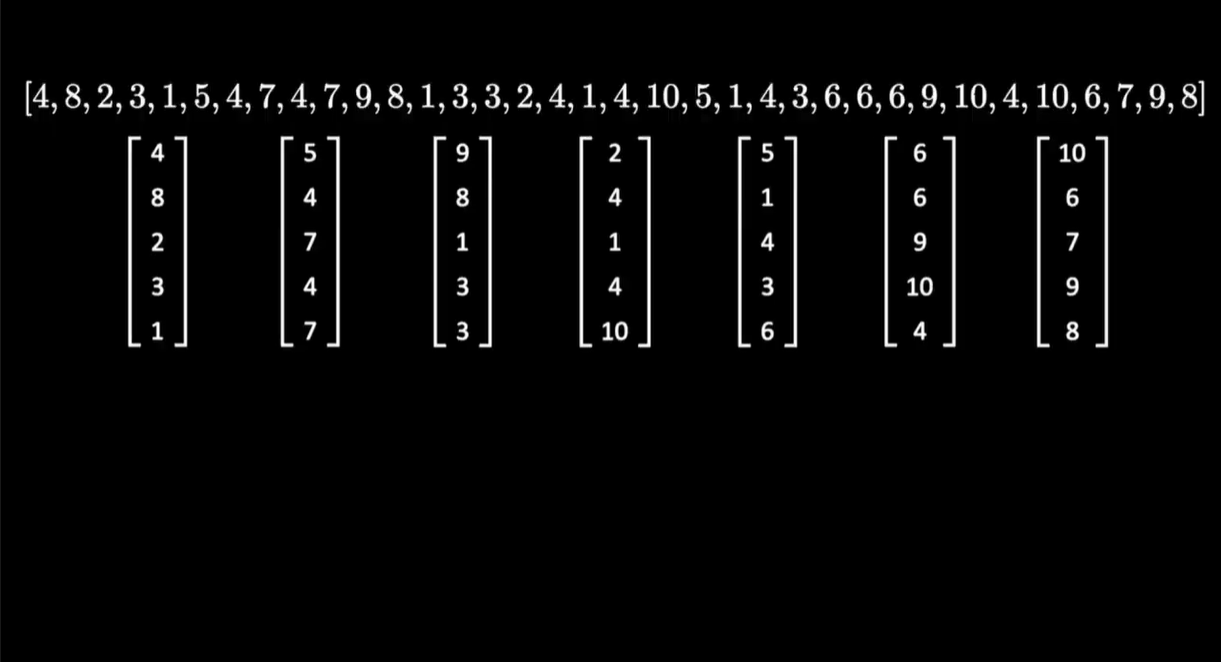
\includegraphics[width=\linewidth]{a.png}}
    \end{center}
\end{frame}

\begin{frame}
    \frametitle{Randomized Select Algorithm}
    \begin{itemize}
        \item Time Complexity:
        \[
        T(n) = c\left(\frac{n}{5}\right) + T\left(\frac{n}{5}\right) + T\left(\frac{7n}{10}\right)
        \]
        \item Explanation:
        \begin{itemize}
            \item \(c\left(\frac{n}{5}\right)\): Time taken to sort all the groups of size 5 and finding their medians.
            \vspace{0.4cm}
            \item \(T\left(\frac{n}{5}\right)\): Time taken to recursively find the median of medians from the array of medians.
            \vspace{0.2cm}
            \item \(T\left(\frac{7n}{10}\right)\): The next recursive call to the randomized select algorithm, which processes at most \( \frac{7n}{10} \) elements, based on the partitioning.
        \end{itemize}
        
    \end{itemize}
\end{frame}
\begin{frame}
    \frametitle{Convex Function}
    \vspace{0.3cm}

    \begin{columns}
        \column{0.6\textwidth}
        \begin{block}{Definition of a Convex Function}
            If $f$ is convex and $0 \leq t \leq 1$, then:
            \begin{itemize}
                \item $t \cdot f(a) + (1-t) \cdot f(b)$ represents a line segment.
                \item For \( \forall a \leq x \leq b \), if the line segment lies on or above $f(x)$:
                \[
                f(a+b) \geq f(a) + f(b) \tag{Eq. 1}
                \]
            \end{itemize}
            \textit{This will be proven by the professor in the next class. For now, we assume it to be true.}
        \end{block}

        \column{0.4\textwidth}
        \centering
        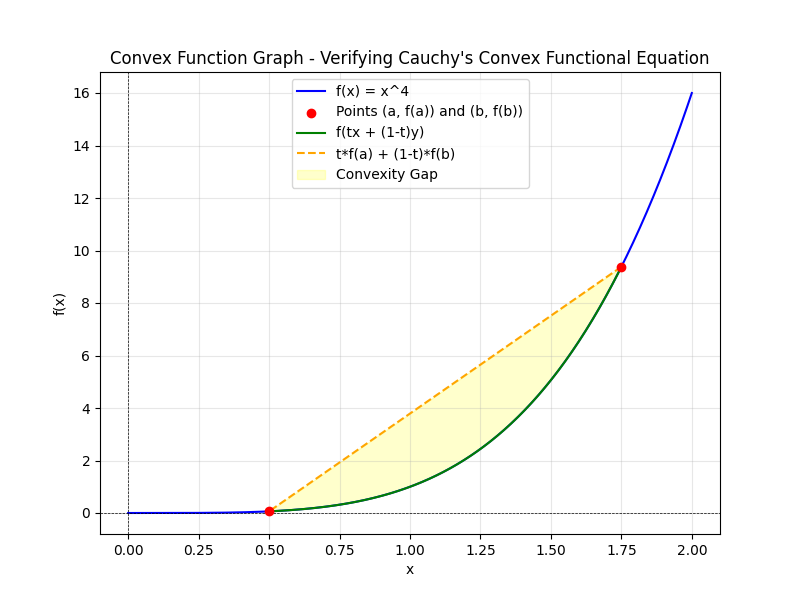
\includegraphics[width=\linewidth]{convex.png}
        
    \end{columns}
\end{frame}
\begin{frame}
    \frametitle{Simplification}
    \section*{Recurrence Analysis}
    \vspace{0.3cm}
        Using Eq. (1), we can simplify as follows:
        \[
        T\left(\frac{n}{5}\right) + T\left(\frac{7n}{10}\right) \leq  T\left(\frac{n}{5} + \frac{7n}{10}\right) \hspace{0.1cm} or \hspace{0.1cm} T\left(\frac{9n}{10}\right) 
        \]
        Therefore:
        \[
        T(n) \leq c\left(\frac{n}{5}\right) + T\left(\frac{9n}{10}\right) 
        \]

        Expanding recursively:
        \[
        T(n) \leq c \cdot \frac{n}{5} + c \cdot \frac{n}{5} \left(\frac{9}{10}\right) + c \cdot \frac{n}{5} \left(\frac{9}{10}\right)^2 + \dots
        \]

        
\end{frame}
\begin{frame}
 \frametitle{Simplification}
The sum can be expressed as:
        \[
        \sum_{i=0}^{\infty} c \cdot \frac{n}{5} \left(\frac{9}{10}\right)^i
        \]
        Factoring \( c \cdot \frac{n}{5} \), we get:
        \[
        T(n) = c \cdot \frac{n}{5} \sum_{i=0}^{\infty} \left(\frac{9}{10}\right)^i
        \]
Using the formula for the sum of an infinite geometric series:
\[
\sum_{i=0}^{\infty} r^i = \frac{1}{1-r}, \quad \text{where } r = \frac{9}{10}
\]

We get:
\[
= c \cdot \frac{n}{5} \cdot \frac{1}{1 - \frac{9}{10}}
\]

Simplifying further:
\[
= c \cdot \frac{n}{5} \cdot 10 = c \cdot 2 \cdot n = O(n)
\]

\end{frame}




\begin{frame}
    \frametitle{Conclusion}
    \begin{itemize}
        \item Recurrence Relations:
        \[
        T(n) = cn + T(|L|)
        \]
        \item Randomized Selection:
        \begin{itemize}
            \item Median-of-medians selection guarantees linear time.
        \end{itemize}
        \item Convex Functions:
        \begin{itemize}
            \item Useful for bounding and analyzing recurrences.
        \end{itemize}
    \end{itemize}
\end{frame}







\begin{frame}
    \frametitle{Homework}

    \begin{itemize}
        \item If the list was not distinct, then what should be done? \vspace{0.4cm}
        \item What is important about chunks of size 5? For example, try sizes 3 and 7. \vspace{0.4cm}
        \item What is the time complexity of the algorithm if we were to make chunks of size $\sqrt{n}$?
    \end{itemize}

\end{frame}



\end{document}
